%\documentclass{UUThesisTemplate}
%\begin{document}
%CECI est un CITE \cite{Butler1921}\\
%CECI est un CITEp \citep{Butler1921}\\
%CECI est un CITEt \citet{Butler1921}\\
%\\
%CECI est un CITE \cite[p.1]{Butler1921}\\
%CECI est un CITEp \citep[p.1]{Butler1921}\\
%CECI est un CITEt \citet[p.1]{Butler1921}\\
\chapter{\label{chap3}Background}%
This chapter provides background information on rhetoric, rhetorical figures and our three figures of speech from the perspective of literary analysis and computational linguistics. This review does not attempt to cover all relevant issues and is by no means exhaustive. Instead, we focus the discussion primarily on aspects that have some bearing on Papers~I–IV.

\section{Rhetoric}
One cannot talk about figures of speech without invoking their antique theoretical framework. The concepts for the figures of speech have their historical roots in the field of rhetoric, whose aim is to teach speakers to convince and persuade their audience. 
The most fundamental notions of rhetoric were defined by Aristotle \citep{Roberts2004} as follows:

\begin{quotation}
Of the modes of persuasion furnished by the spoken word, there are three kinds. The first kind depends on the personal character of the speaker [ethos]; the second on putting the audience into a certain frame of mind [pathos]; the third on the proof, or apparent proof, provided by the words of the speech itself [logos]. Persuasion is achieved by the speaker’s personal character when the speech is so spoken as to make us think him credible.
   –Aristotle 1356a 2,3 (Translated by \cite{Roberts2004})
\end{quotation}
\noindent
In this extract, Aristotle gives three key notions to explain the mechanisms involved when trying to persuade someone. One can act on the ethos, which is the way one gives credit to the speaker. Then one can act on the pathos, that is, the appeal to the emotion of the audience. Finally one can act on the logos, which in Greek means both logic and discourse, and which can be defined as the way one articulates the ideas, the reasoning. While Aristotle preferred that arguments be based as much as possible on logos, he did pay considerable attention to the appeal to emotion, and discussed it extensively in his \textit{Rhetoric}.


Ancient authors such as Hermogenes and Quintilian \citep{Butler1921} were passionate about rhetoric and not only practised it but also tried to define and model it. They observed patterns of discourse that would benefit their argumentation. Among those patterns are the ornaments called figures of speech, also known as rhetorical figures. In his Oratio  \citep{Butler1921} Quintilian tries to describe all the figures. His classification still inspires works of classification today \citep{harris2009,Burton1996}. This classification is not uncontroversial.  Indeed, the notion that figures of speech are additional ornaments that deviate from a ``normal'' way to express things has been repeatedly questioned in modern linguistics and philosophy \citep{Jakobson1956,Derrida1982}.%[white mythology]
 
 Figures of speech can, in fact, leverage any of the appeals identified by Aristotle (logos, pathos, ethos). In an extensive work of classification, \cite{Howard2010} tries not only to define each figure of speech but also to label them with the appeal they are used for. For instance, he says that chiasmus and epanaphora appeal to logos and pathos. That can be a subject of controversy. For instance, \citet{Vandendorpe1991} seems to criticise some examples of chiasmi for acting merely on the impression made by the author, and by extension the ethos. Indeed, for him, this figure is an over-sophisticated way to express what sometimes are very cliché ideas (for example, ``the research of the meaning is the meaning of research''). Thus, for \citet{Vandendorpe1991}, this extreme ability to play with words could make the audience give too much credit to the speaker by thinking that he or she is clever. As we will see in \Cref{secDef}, rhetorical figures are vaguely defined, and this is just one example of the controversies raised by this topic.

% In distinguishing schēma from trope, Quintilian calls it “a purposeful deviation in sense or language from the ordinary simple form; the analogy is now with sitting, bending forwards, or looking back” ( Institutio oratoria . Later analogies reinforce this distinction between inward meaning and outward form by comparing schemes to costume, clothing, and ornament. Cl. definitions of scheme thus rely on an idea of ordinary (naked, natural, or plain) speech that is then clothed by the figures of rhet. The discursive force of such *ornament varies throughout rhet.’s long hist., with schemes swelling in number and acquiring greater currency in courtly cultures that emphasize fashion, performance, or external show as constitutive of identity. In theories of rhet. and poetics informed by mod. ling., there is considerable skepticism toward the notion that there exists an “ordinary” lang. to be ornamented by figures of speech. Such theory concludes that rhetorical figures are not supplementary decorations but rather fundamental structures of lang. and thought ( Jakobson, Derrida, de Man). Although this theory of figures as constitutive of, and coextensive with, lang. makes its exemplary arguments with reference to tropes such as *metaphor and *metonymy, it has resulted in a generalized critical method inclined to discover substantive meaning in the lexical patterns and shapes of what used to be called rhetorical schemes. See figuration, linguistics and poetics, rhetoric and poetry. ᭿ Jakobson and Halle, “Two Aspects of Language and Two Types of Aphasic Disturbances”; E. Auerbach, “Figura,” trans. R. Manheim, Scenes from the Drama of European Literature (); O. Ducrot and T. Todorov, Encyclopedic Dictionary of the Sciences of Language , trans. C. Porter (); G. Genette, Figures of Literary Discourse , trans. A. Sheridan (); T. Todorov, Introduction to Poetics , trans. R. Howard (); de Man, “The Rhetoric of Temporality” and “The Rhetoric of Blindness”; P. de Man, “Anthropomorphism and Trope in the Lyric,” The Rhetoric of Romanticism (), and “Hypogram and Inscription” and “The Resistance to Theory,” The Resistance to Theory (); J. Derrida, “White Mythology,” Margins of Philosophy , trans. A. Bass (); Vickers, Defence ; B. Dupriez, A Dictionary of Literary Devices (); Lanham; Renaissance Figures of Speech , ed. G. Alexander, S. Anderson, and K. Ettenhuber (); G. Burton, “Silva Rhetoricae,” http://rhetoric. byu.edu. J. C. Mann SCHOOL OF SPENSER. A group of Eng. poets of the earlier th c., strongly under the influence of Edmund Spenser (– ). Their work is sharply distinguished from the more radical poetic movements of the time, epitomized by the *classicism of Ben Jonson and the *metaphysical style of John Donne. The principal poets of the Spenserian school—William Browne of Tavistock, Michael Drayton, George Wither, Giles and Phineas Fletcher, and the Scottish poets William Drummond of Hawthornden and Sir William Alexander— show the influence of Spenser in their sensuous imagery, smooth meter, archaic *diction, and fondness for narrative and *pastoral modes of expression. They also owe to Spenser their allegorical and moral tendencies. Such ambitious narrative poems as Giles Fletcher’s Christ’s Victory and Triumph and Phineas Fletcher’s The Apollyonists suggest Spenser’s Faerie Queene in their pictorial quality and their stanza forms (modified *Spenserian stanzas); they also anticipate John Milton, who, occasionally echoing the Fletchers, followed them in the use of Christian material for epic purposes and who himself acknowledged his indebtedness to Spenser, whom he called master . ᭿ H. E. Cory, Spenser, the School of the Fletchers, and Milton (); D. Bush, English Literature in the Earlier Seventeenth Century, –  , d ed. (); J. Grundy, The Spenserian Poets (); The English Spenserians, ed. W. B. Hunter Jr. ()—anthol.; P. J. Finkelpearl, “John Fletcher as Spenserian Playwright: The Faithful Shepherdess and The Island Princess ,” SEL  (); M. Quilligan, Milton’s Spenser (); G. M. Bouchard, “Phineas Fletcher: The Piscatory Link The Princeton Encyclopedia of Poetry and Poetics : Fourth Edition, edited by Stephen Cushman, et al., Princeton University Press, 2012. ProQuest Ebook Central, .Created from uu on 2017-09-28 07:40:08. 
%Previous extract from "scheme" in greene.
% is still inspiring works on classification of today \citep{harris2009,Burton1996}. Although the all notion of figures of speech as simple additional ornament that would deviate to a somewhat `normal' way to express things is abundantly questioned by the contemporary linguistics framework \citep{Jakobson1956},\citep[White Mythology]{Derrida1982}.
 
% Figures of speech can in fact leverage any of the appeals defined by Aristotle (logos, pathos, ethos). In an extensive work of classification \cite{Howard2010} tries not only to define each figures of speech but also to label them with the appeal it is used for. For instance he says that chiasmus and epanaphora appeals to logos and pathos. That can be subject of controversies as \citep{Vandendorpe1991} seems to criticise some examples of chiasmus for acting merely on the image given by the author, so by extension the ethos. Indeed, for him, this figure is an over sophisticated way to express an idea sometimes very cliché (i.e. `The research of the meaning is the meaning of research'). Thus for \citet{Vandendorpe1991} this extreme ability to play with word could push the audience to give too much credit to the speaker by thinking that he or she is clever. As we will see in \Cref{secDef} rhetorical figures are vaguely defined and, this is just one example of controversy raised up by this topic.
 
\section{Rhetorical Figures\label{secDef}}
\subsection{Schemes and Tropes}
\keyn{Figures of speech}, also called \keyn{rhetorical figures}, are commonly divided into two categories,  \keydef{tropes} and \keydef{schemes}. This separation between figures of speech comes from the classification of Quintilian \cite[p.196]{fahnestock1999}. 

A trope is defined as:
\begin{quotation}
An artful deviation from the ordinary or principal signification of a word. \\\citep{Burton1996}%\footnote{http://rhetoric.byu.edu/Figures/Tropes.htm}
\end{quotation}
\noindent
Tropes such as “the Lord is my shepherd” (metaphor), “the pen is mightier than the sword” (metonymy), and “the face that launched a thousand ships” (synecdoche) operate by changing the signification of the words ``shepherd'', ``pen'', ``sword'', and ``face''. %Thus, tropes allow language to mean more or something new.% \citep[Art. Trope]{greene2012}. 


\cite{greene2012} define a scheme as a change in standard word order or patterns. This includes any artful deviation from the ordinary arrangement of words. Unlike tropes, which work on the signification of words, schemes involve their arrangement \citep[Art. ``Scheme'']{greene2012}.  For instance an enjambement can be considered as a scheme. It is defined as an unnatural ``cut'', which can result in stylistic effects (emphasis, contrast, double interpretations) (see \Eref{exEnjamb}).
\nnumsentence{I’d rather\\
be naked \\
of fake friends\label{exEnjamb}}%\vspace{-18pt}
%
Beneath the category of schemes, there are many subcategories. Among them are the categories of repetitive figures or figures of repetition, which include every figure involving repetition of linguistic units such as letters, words or concepts.
 This is where chiasmus, epanaphora and epiphora belong. Depending on the sources, their number can vary, as will be explained for the case of chiasmus (\Cref{secChiasmus}). As for now, we can say that there is no one unique way to name and categorise figures. We are not going to list all figures of repetition,\footnote{For an extended list of repetitive figures, we refer the reader to \url{http://rhetoric.byu.edu/Figures/Groupings/of\%20Repetition.htm}. } but we can present three clear examples that are representative of what repetitive figures can be.
 \begin{itemize}
  \item Alliteration: Repetition of initial or medial consonants in two or more adjacent words.
  \item Anadiplosis: Repetition of a word at the end of a clause and then at the beginning of the succeeding clause.
%\item Assonance: Repetition of similar vowel sounds, preceded and followed by different consonants, in the stressed syllables of adjacent words.
 \item Antanaclasis: Repetition of a word in two different senses.
 \end{itemize}
Another controversy that has some bearing on our work concerns whether a figure of speech (trope or scheme) should be considered only if it is \keydef{intentional} or, in other words, is intended by the author. Such a definition of figures of speech, used in some computational linguistics work \citep{Strommer2011}, causes a problem in the literature field.\footnote{The status of the author has been widely questioned in both 20th-century and contemporary literary theory \citep{Barthes1984}. Indeed, it is argued that no one can really pretend to know the intention of the author. We are aware of this controversy but will not address it here.} For this reason we avoid focusing too closely on the term ``intentional'' because we do not want to fall into any author fallacy. This choice will be reflected in how we formulate our questions during the annotation process (see \Cref{secHowAnnot}).  %, and it is certainly not our role to say if it is true or not.} 

%As far as we are concerned, the debate on intentionality is of limited relevance for this thesis. Indeed
%, de facto when we will annotate examples, 
%we will be dependent on what is our own interpretation as a reader. This perception can vary between annotators. Thus, we choose to avoid the term `intention' because it would suggest that we pretend to know the auctorial intention and that we limit text interpretation to what the author meant. 
%The important thing to explain here is how this can impact our task concretely. 
%this theoretical assumption, most of the time, will not significantly change the system we develop as we focus the task on detecting the most prototypical cases. After all, when someone quotes `Fool is fair and fair is fool', whether you read this sentence from the supposed point of view of the author or from the perception of the reader, the conclusion should be the same: we are in the presence of a chiasmus. It is only in some borderline cases that our theoretical position has impact. 
%%%%%%EXAMPLE REMOVED%%%%
%\footnote{Let us take this exceptional but real example extracted from a French book:
%
%\nnumsentence{he \mn{regifies} the \mn{stars} and \mn{starifies} the \mn{kings} \label{exStar}}
%
%When looking at this example, some users will never see any chiasmus. However, some others, if they have studied latin, will argue that `regifies' comes from the Latin `rex/regis' which means king;  thus there is a chiasmus playing on the notions of `king' and `star'. If we take the auctorial point of view, we will have to document ourselves and see if the author has studied latin and conclude if he/she is likely to have intended this chiasmus. However, if we abandon the idea of looking for what was the intention of the author, we can consider that this chiasmus does not exist in the eyes of most readers because most readers are non-latinist.} 
%And in reality, we will see in Chapter~4 by comparing the results of our exploration on epanaphora with the ones of \citet{Strommer2011} that we have reasons to believe that this theoretical choice does not impact dramatically the number of candidates we consider as real instances of rhetorical figures. 

In this first part, we have given a general overview of what rhetoric is and how rhetorical figures can be defined. We have touched on aspects of the theoretical debate that can be relevant to our approach to detection. In the next section, we give a definition of the three figures we are studying. One figure, however, will be studied more extensively: chiasmus. Throughout this study, we will see how multiple challenges already arise when searching for a definition and a list of terms adapted to the requirements of computational linguistics.\clearpage

\subsection{Chiasmus}
\label{secChiasmus}
The word ``chiasmus'' comes from the Greek letter $\chi$ because of the cross this letter symbolises. Indeed, chiasmus is generally defined as the reuse of a pair of elements in reverse order, as in Figure~\ref{crossSchem1}.
\vspace{0.2cm}%
\begin{figure}[H] 
\begin{center}
%\resizebox{0.1}{0.1}{
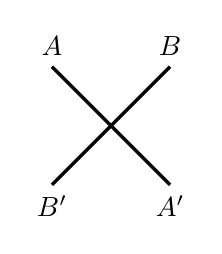
\begin{tikzpicture}[scale=1.5]
\draw [very thick]  (0,1.5) node[above]{$A$} -- (1,0.5) node[below]{$A'$};
\draw [very thick]  (0,0.5) node[below]{$B'$} -- (1,1.5) node[above]{$B$};
\end{tikzpicture}
%}
\end{center}
\vspace{-0.3cm}
\caption{The chiasmus schema \label{crossSchem1}} 
\end{figure}
\vspace{-0.5cm}
\begin{figure}[h!] 
\begin{center}
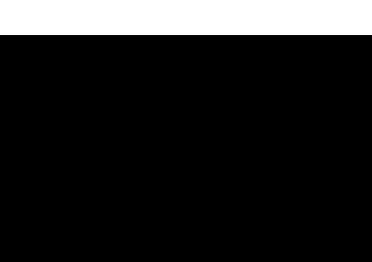
\includegraphics[scale=0.5]{images/X}
\vspace{-0.4cm}
\caption{A chiasmus example\label{graphX}}
\end{center}
\end{figure}%
\vspace{-0.1cm}
\noindent
There are many forms of chiasmus. They can consist of cross-like arrangements of phonemes, letters, or syntactic elements. We will focus on the chiasmus of words, also called antimetabole. However, even within this single subcategory, we observe many variations that we need to define for the automatic treatment \citep{gawr}. As a result of this, we present the types of chiasmus of words that we have identified.\footnote{This typology is inspired by and adapted from the one developed in French by \cite{dubremetz2013}.} This typology was obtained by reading a number of
definitions given in the literature \citep{Diderot1789,gradus,garcia,greene2012,larousse,Nordahl1971,
rabatel,Vandendorpe1991,VanGorp2001} and observing what kinds of examples they are citing.
\clearpage
%Il existe toute sorte de chiasmes, ils peuvent porter sur le croisement de phonèmes, de lettres, d'éléments syntaxiques... Nous nous restreindrons à l'étude des chiasmes de mots. Cependant on constate dans cette sous-classe de chiasmes encore beaucoup de variantes qu'il faut définir pour le traitement automatique \cite[p.67]{gawr}.  Voici donc, à l'issue des lectures des linguistes \footnote{ \citet{Diderot1789,gradus,garcia,Greene2012,Nordahl1971,larousse,rabatel,Vandendorpe1991,VanGorp2001}} et de l'observation des exemples qu'ils donnent, les types de chiasmes de mots que nous avons recensés :



%\begin{table}[H]
%\begin{savenotes}\label{tablSynthDef}
%%=============TABLEAU=========
%\begin{tabular}{|b{1.5cm}|p{2cm}|p{3cm}|p{3cm}|p{3cm}|}
%\hline
% & \multicolumn{2}{c|}{\textbf{Name}} & \textbf{Repeted Elements:} &\textbf{\ \ \ \ \ \ \  Example}\tabularnewline
%\hline 
%\hline 
%	\multirow{30}{1.5cm}{
%	\begin{center}\textbf{Chiasmi of words}%\\\\\\\
%%========FIGURE=========
%\begin{figure}[H]
%\ \ \ \begin{tikzpicture}[scale=0.4]
%\draw [very thick]  (0,1.5) node[above]{$A$} -- (1,0.5) node[below]{$A'$};
%\draw [very thick]  (0,0.5) node[below]{$B'$} -- (1,1.5) node[above]{$B$};
%\end{tikzpicture}
%%\caption{Schéma définitoire du chiasme} \label{crossSchem1}
%\end{figure}
%%========FIGURE=========
%	\end{center}} 
%
%%	%=====première entrée=====
%		 	& \multicolumn{2}{p{3cm}|}{\begin{center}Antimetabole or Strict antimetabole\end{center}} 
%		 	&\begin{center} identical words / pair of strings \footnotemark{\cite[Art."Chiasme"]{gradus, larousse}}  \end{center}
%		 	& \textit{\textit{\mn{Sounds} of \mn{poetry}, and \mn{poetry} of \mn{sounds}.}%(Shakespeare)
%		 	} \tabularnewline
%	%!=====deuxième entrée=====
%			\cline{2-5} 
%	%=====troisème entrée=====
%		 & \multicolumn{2}{p{3cm}|}{\begin{center}Flexional chiasmus or Flexional antimetabole\end{center}}  
%		 & \begin{center}
%inflected lemmas
%\end{center}
%		 & \textit{An optimist \mn{laughs} to \mn{forget}, a pessimist \mn{forgets} to \mn{laugh}.} %(Anonymous)
%		 \tabularnewline
%	%=====troisème entrée=====
%		\cline{2-5} 
%	%=====quatrième entrée=====
%		 & \multicolumn{2}{p{3cm}|}{\begin{center}Derivational chiasmus\end{center}} 
%		 & \begin{center}derived stems \end{center}
%		 &\textit{ \mn{Modernise} \mn{Islam} rather than \mn{islamisation} of \mn{modernity}.} %(Jean Daniel)
%		 \tabularnewline
%	%=====!quatrième entrée=====
%		\cline{2-5} 
%	%=====cinquième entrée=====
%		 & \multicolumn{2}{p{3cm}|}{\begin{center}Antimetalepse\end{center}} 
%		 & \begin{center}
%Idea or notion but without necessarily reusing morphologically related words \footnote{\cite[Art. "Antimétabole, Antimétalepse, Antimétathèse"]{Diderot1789}} 
%\end{center}
%		 &  Who \mn{dotes}, yet \mn{doubts}; \mn{suspects}, yet \mn{loves}.%---Othello
%		 \tabularnewline
%	%!=====cinquième entrée=====
%\hline
%\end{tabular}\end{savenotes}
%\caption{Typology of chiasmus of words\label{tabTypo}}\end{table}

%%%%%%%%%%%%%%%%%%END TABLEAU

\begin{table}[H]

\begin{savenotes}\label{tablSynthDef}
\footnotesize

%=============TABLEAU=========
\begin{tabular}{|c|c|c|}
\hline
\textbf{Name} & \textbf{Repeated Elements} &\textbf{Example} \\
\hline 
Antimetabole or & Identical word forms\footnotemark[4] & \mn{Sounds} of \mn{poetry},  \\
Strict antimetabole & (pair of strings) & and \mn{poetry} of \mn{sounds}.\\
\hline 

Flexional chiasmus or & Inflected lemmas & An optimist \mn{laughs} to \mn{forget},  \\ %(Anonymous)
Flexional antimetabole & & a pessimist \mn{forgets} to \mn{laugh}. \\
\hline 
Derivational chiasmus & Derivations with same stem & \mn{Modernise} \mn{Islam} rather than \\ %(Jean Daniel)
& & \mn{islamisation} of \mn{modernity}. \\
\hline 
Antimetalepse & Ideas or notions, but without & Who \mn{dotes}, yet \mn{doubts}; \\%---Othello
& necessarily reusing  & \mn{suspects}, yet \mn{loves}. \\
& morphologically related words\footnotemark[5] & \\
\hline
\end{tabular}\end{savenotes}

\caption{Typology of chiasmus of words\label{tabTypo}}\end{table}



\footnotetext[4]{\cite[Art."Chiasme"]{gradus, larousse}}
\footnotetext[5]{\cite[Art. "Antimétabole, Antimétalepse, Antimétathèse"]{Diderot1789}}
\setcounter{footnote}{5}


 Even if the term chiasmus is a recent one,\footnote{This term does not appear until the second half of the 19th century \cite[p. 24]{horvei1985}.} the figures described in this table are very old and have been known for a long time. For instance, already in Quintilian we observe the existence of antimetabole of identical terms but with different inflexions, though no name has ever been given to this phenomenon to differentiate it from the strict antimetabole. A similar lack of defining terms is noticeable for the chiasmi that allow derivations.
 This table is probably not exhaustive and it is dependent on the examples cited as canonical in the literature. It should not be seen as the sole possible classification of chiasmus and antimetaboles. In fact, some authors prefer to refer to antimetabole as reverted antithesis \citep{Viklund2002}. Others, by contrast, want to consider those special cases a completely different figure called ``reversion'' \cite[Art. Reversion]{font}.\footnote{We can trace this back to another conflicting classification in Antiquity, as Hermogenes prefers to place chiasmus under a category of figure completely separated from other figures of repetition. For him chiasmus belongs to ``gorgotes'' (i.e.,``vigour''), whereas epanaphora and epiphora are a sort of parallel figures that should be placed under ``kallos'' (i.e., ``beauty'') \citep{Wooten2012}.}   
 As stated by \cite[p. 3]{Watson1912}:
\begin{quotation}
 The importance attached to rhetorical expression among ancient writers is recognized not only by special treatises written by them, but in the compilations or writings on rhetoric by modern authors who have made special study of such treatises. These ancient writers discuss in bewildering profusion examples with subdivisions of tropes, figures of rhetoric, figures of syntax, etc. But frequently their definitions do not offer a basis for clear cut division. Hence it is often impossible to make any sharp or important distinction between tropes, figures rhetorical, and figures grammatical, and no two writers of the present day arrange them in exactly the same way.
\end{quotation}
\noindent
 Thus we see \Cref{tabTypo} as one possible classification that answers our specific problem of defining the task for a computer. %It will allow us to progress towards the definition of the task to be carried out by the computer. 
 Indeed without a clear, formal and adapted definition, it will be difficult to make any system of detection \cite[p. 67]{gawr}.
 
%  \cite[Art. Antimétabole]{Greene2012} l'existence des antimétaboles comportant des mots identiques mais aux flexions différentes. Cependant jamais un nom spécifique n'a été donné à ce phénomène pour le différencier de l'antimétabole stricte. Il en va de même pour le chiasme portant sur des mots dérivés.
%Ce tableau n'est sans doute pas exhaustif puisqu'il est tributaire d'observations empiriques à partir des exemples donnés par les ouvrages de stylistique de référence. Il va cependant permettre à cette recherche d'aller plus loin et de ne pas se heurter au flottement {}\cite[p.21]{rabatel} qui règne autour de la définition de cette figure : car sans définition formelle, il s'avère difficile d'élaborer un système de détection \cite[p.67]{gawr}.





%The chiasmus of words, also called antimetabole, is defined as the repetition of a pair of words in reverse order. %The term chiasmus of words, sometimes called antimetabole, consists in the reuse of a pair of words in reverse order for a rhetorical purpose. 
%It is called `chiasmus' after the Greek letter $\chi$ because of the cross 
%this letter symbolises (see Figure~\ref{graphX}).
% %======Schéma=======
%\begin{figure}[h!] 
%\begin{center}
%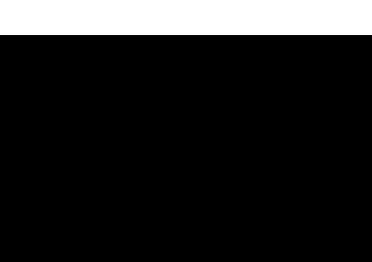
\includegraphics[scale=0.5]{images/X}
%\caption{Schema of a chiasmus}
%\label{graphX}
%\end{center}
%\end{figure}

From now on, we will restrict the term `‘chiasmus’' to cases based on identity of lemma  (i.e., flexional chiasmus in \Cref{tabTypo}). This restriction is a compromise aiming to make the task feasible. Indeed, if we tried to detect all kinds of chiasmus, technical difficulties would pile up  that would prevent any deep investigation. For example, the extraction process would become noisier and we would have to improve stemmers as well as ontologies \citep{dubremetz2013}.

In this part we have investigated the definition(s) of chiasmus, and have proposed a typology. This typology divides chiasmi into different subtypes based on similarities between words, and can differ from some authors' definitions partly because there is a lack of consensus about what kind of figure each name should denote. This does not however mean that we completely ignore other definitions. In fact, we consider those other definitions to be observations about the figure behaviour, which provides a precious help in designing features. For instance, in \Pref{paper1}, we decide to use negations like ``not'' in order to capture chiasmi based on antithesis. In \Pref{paper2} we decide to model switching of  syntactic roles between main words in order to model the notion of symmetry described by \cite{morier}.

When we get to the actual experimentation in this thesis, the definition of a candidate chiasmus will be limited as follows:
\bigskip
\begin{enumerate}
\item A chiasmus is the repetition of a minimum of two pairs of words in reverse order satisfying the ABB$\textprime$A$\textprime$ schema, as in \Cref{crossSchem1}.
\item The words repeated should appear within a reasonably limited context. In our actual implementation: 30 tokens.\footnote{30 tokens is the upper bound found empirically by \citet{dubremetz2013}. In that corpus study, the largest chiasmus found consisted of 23 tokens.}
\item The word pairs (AA$\textprime$ and BB$\textprime$) should have the same lemma.
\end{enumerate}
%Despite a long tradition in rhetorics and linguistics, the terms {\em chiasmus} and {\em antimetabole} do not really have clear definitions. In the earliest times, \citet{Diderot1789} as well as Quintilian \citep{Greene2012} give us very basic identification features. They talk about the degree of identity that can be accepted to consider two words as identical (strictly identical strings, lemmas or synonyms). Finally, \citet{rabatel} and \citet{Nordahl1971} try to find subcategories of chiasmi on a deep semantic basis: for instance chiasmi expressing contrast \cite{rabatel}. %The notion of antimetabole is floating. Dictionaries of stylistics tend to quote the same prototypical chiasmi to illustrate examples, which is not helpful when trying to capture the linguistic variety of chiasmi.



\subsection{Epanaphora}
The lack of definitions adapted to computational linguistics is not exclusive to chiasmus. In fact, any figure of speech suffers from a lack of consensus about the definitions, or from vagueness in delimiting what we are looking for. Epanaphora confirms this rule.
Epanaphora\footnote{In rhetoric, \emph{epanaphora} is better known under the competing term \emph{anaphora}. However, in computational linguistics the term \emph{anaphora} can be ambiguous, as it also refers to a referential pattern. For the sake of clarity, we will only use the term \emph{epanaphora}.}
 is defined as the repetition of a word or a group of words at the beginning of several sequences of language. Curiously, the ambiguity in the definition of epanaphora does not concern the same issue as for chiasmus. For chiasmus it is the type of element that can be criss-crossed (sounds, letters, strictly similar words or just synonyms) that is unclear. For epanaphora there seems to be some kind of consensus: only words should be the object of the repetition (not letters or sounds). And all examples cited by our references were concerned with repetition of words that at least share the same lemma. Where the definition gets blurry is: (1) What type of sequences should be considered? (2) How close together should they be? 

Regarding the first question, ``sequences'' can be defined in different ways. One can speak of epanaphora of paragraphs \citep[Art. L'anaphore et l'épiphore]{Bacry1992}, verses \citep[Chap. III]{Suhamy2004}, clauses or phrases \citep[Art. Anaphore]{gradus}. All authors have at least invoked or cited in their examples the sentence as a possible sequence for epanaphora production. In addition, sentence splitting is a nearly solved problem in natural language processing. Sentences should not represent a major challenge for definition and extraction. That is why, in this thesis, we limit the scope to epanaphora of sentences, as exemplified in  Example~\ref{exIam}. 
%
\nnumsentence{\mn{I am} an actor.\newline
\mn{I am} a writer.\\
\mn{I am} a producer.\\
\mn{I am }a director.\\
\mn{I am }a magician. \label{exIam}}%
%
On the second question, some authors, like \citet[Chap. III]{Suhamy2004} and \citet[Art. L'anaphore et l'épiphore]{Bacry1992}, talk about ``successive'' sequen\-ces, while others seem to consider repetitions that skip one or several sequences before producing a repetition to be an epanaphora \cite[p.329]{font}. To keep the problem simple, we will consider only epanaphora relying on immediately successive sentences.

%  \enumsentence{\mn{We shall }not flag or fail.\\ \mn{We shall} go on to the end.\\ \mn{We shall} fight in France [\ldots].\\ \mn{We shall} never surrender.  \label{exWeShall}}

As for chiasmus we limit the definition of candidate epanaphora as follows:

\begin{enumerate}
\vspace{0.2cm}
\item An instance of epanaphora consists of two or more adjacent sentences.
%
\item One or more words are repeated at the beginning of each sentence.\footnote{We started our exploration by requiring at least one word, but for feasibility we later had to restrict it to at least two words (see \Pref{paper4}).}%\footnote{This constraint is applied during exploration part. Following this exploration, for feasibility purpose, we had to restrain this limit to 2 words at the beginning of the sentence (see, \Pref{paper4}).}
\item To count as repetitions, the words should have the same lemma.\footnote{As for the previous constraint, we have later restricted it to a strict identity of word or string chain.}
%\item The sentences should follow each others and should not be cut by another sentence not repeating the first term.
\end{enumerate}
\subsection{Epiphora}
Epiphora\footnote{Epiphora is also known under the term \emph{epistrophe}, but for consistency with \emph{epanaphora} we will only use the term \emph{epiphora}.} is a figure of speech with repetition at the end of a sequence (see Example~\ref{exGullible}).
%
\nnumsentence{
I'm so \mn{gullible}.\\
I'm so damn \mn{gullible}.\\
And I am so sick of me being \mn{gullible}. \label{exGullible}%
}%
%
%\enumsentence{For everyone who \mn{exalts} himself will be \mn{humbled}, and everyone who \mn{humbles} himself will be \mn{exalted}. \label{exhumble}}
\noindent
As for epanaphora, one speak of epiphora of paragraphs, lines, clauses or phrases, but as with epanaphora we limit the scope to sentences, as exemplified in  Example~\ref{exGullible}.
Epiphora is usually defined as merely epanaphora in reverse. In most of the sources that we have consulted \citep{Bacry1992,greene2012,Suhamy2004,gradus,font}, this term does not even have a separate paragraph. There could be several reasons for this; perhaps its theoretical proximity to epanaphora makes it not useful to study this figure on its own. Perhaps those authors also suffer from a lack of examples to refer to. Indeed, one author \citep{Bacry1992} claims that this figure is less frequent than its counterpart. He argues that the repetition of epanaphora is more visible than any other repetition because it is placed first. He assumes that this visibility makes this figure more popular. \cite{Bacry1992} also seems to look for some specific property that would distinguish epiphora from epanaphora. For instance, he thinks that epiphora is less violent than epanaphora, and that it is particularly suitable in the context of melancholia.\footnote{For an example of epiphora in the context of melancholia the reader can refer to the poem ``The Raven'' by Edgar Allan Poe \citep{poe1898raven}.}
As with chiasmus and epanaphora, we limit the definition of candidate epiphora:
\begin{enumerate}
\vspace{0.2cm}
\item An instance of epiphora consists of two or more adjacent sentences.
\item One or more words are repeated at the end of each sentence.
%\item The identity shared should be an identity of lemma.
\item To count as a repetition, the words should have the same lemma.
\end{enumerate}

\section{Related Work in Computational Linguistics}
In this section we will give an overview of the work related to our topics. A first part will discuss research targeting a variety of stylistic phenomena related to figures of speech. The second part focuses on one particular figure of speech frequently treated in computational linguistics: metaphor. The last part discusses our three rhetorical devices in the context of computational linguistics.

\subsection{Stylistic Phenomena in Computational Linguistics}

In a study about rhetorical figures, \cite{harris2009} claim:
\begin{quotation}
Too much attention has been placed on semantics at the expense of rhetoric (including stylistics, pragmatics, and sentiment). While computational approaches to language have occasionally deployed the word ``rhetoric'', even in quite central ways (such as Mann and Thompson's Rhetorical Structure Theory \citep{Mann1988a}), the deep resources of the millenia-long research tradition of rhetoric have only been tapped to a vanishingly small degree.
\end{quotation}
\noindent
Reading \cite{harris2009} one might think that natural language processing has only modelled semantic aspects of texts without much consideration for the form. However, this is probably not what they mean. It is certainly true that the use of very specialised terms describing rhetorical figures such as ``antithesis'', ``antimetabole'' or ``elision'' is rare in our community.\footnote{Observation based on key word search results on the ACL anthology \\\url{https://aclanthology.coli.uni-saarland.de}.} However, one should not believe that NLP has totally ignored style and effect. In fact, we believe that a lot of research treats rhetoric in some way that involves figures of speech, but with slightly different focus and/or using different terms to talk about it. For instance, \citet{Booten2016} and \citet{Bendersky2012} work on finding what makes sentences ``quotable''. More precisely, what are the fundamental properties of pieces of text that push Internet users to cite them on specialised quotation websites \citep{Bendersky2012} and on Tumblr under the label ``\#quote'' \citep{Booten2016}? Other researchers talk about ``memorability'' of sentences \citep{Danescu-Niculescu-Mizil+al:12b}. %
There is even work on poetry that asks the question of what makes up the ``quality'' of a poem \citep{Kao2012}, and others that look for how to model ``humour'' in a double entendre \citep{Kiddon2011a}. 

Considering these research studies, we believe that NLP is treating rhetoricity (i.e., how the text produces an effect on the reader through its form, the way it is written), but is exploring it with its own concepts (here, ``memorability'', ``humour'', ``quotability''). There may be several reasons for this, but after doing the research on how to define chiasmus, we definitely believe that rhetorical figures are not easy to define. They suffer from a lack of consensus among rhetoricians and linguists. This is a real obstacle for NLP researchers; even before facing any implementation problem, they need to handle ambiguous definitions in a domain, rhetoric, that they do not feel qualified to discuss. %
This might change in the future with the growing interest in digital humanities. Indeed, in recent years, some work within machine learning has targeted very specific literary concepts such as free indirect speech \citep{hammond2013}, similes \citep{niculae2013}, enjambment \citep{ruiz2017}, or rhymes \citep{Mccurdy2015}. In particular, the studies by \citet{hammond2013} and \citet{Brooke2015}, inspired by other research on subjectivity, like that of \citet{Morris2004}, tend to allow subjectivity, multiplicity of text interpretation and variance in the intensity of the phenomena that they automatically detect.\footnote{See their website on automated analysis of Voices in T.S. Eliot's The Waste Land http://www.hedothepolice.org/. Their division of the poem into voices integrates the degree of confidence by the computer and has directly inspired our method \citep{hammond2013}.} This is an essential feature when analysing literature. %

\subsection{A Particular Case of Trope: Metaphor}
When talking about figures of speech in computational linguistics, the first figure that comes to mind is metaphor.\footnote{According to our research on the key term ``metaphor'' in the ACL Anthology \url{https://aclanthology.coli.uni-saarland.de}, the term definitely stands out with more than 100 articles.}
In this domain, extensive work has been done within from computational linguistics, relying on cognitive science and corpus studies. Metaphor  attracts the attention of computational linguists because it is seen as a massive and recurrent language phenomenon. This cognitive phenomenon \citep{LakoffJohnson80} 
%\cite{ (Lakoff \& Johnson, 1980, 1999)
 commonly appears in language in the form of metaphoric expressions  \citep{Deignan2005}. The most comprehensive manual study of metaphoric expressions in large corpora \citep{Steen2010} found that up to 18.5\% of words in the British National Corpus were used metaphorically. This explains why metaphors are treated to a much greater extent in computational linguistics than any other figure: they are too frequent to ignore. 
Beginning with \cite{Wilks1978}, the issue of metaphor has been approached as an identification task: first look for metaphoric expressions and then (1) prevent them from interfering with the computational treatments of literal expressions and (2) use them to increase the understanding of the content % to gain additional insight about a text 
%to paraph from here:
%
(e.g., \citet{Carbonell1980}, \citet{Neuman2009}). %
The task is generally defined like this: for a given unit of language (e.g., word, phrase, sentence) decide whether it is metaphoric or non-metaphoric. \citet{Neuman2009} used selectional restrictions for this purpose; \cite{Mason2004} used hand-crafted knowledge resources to detect similar selectional mismatches. Another approach is to detect selectional mismatches using statistically created resources (e.g., \citet{Shutova2013a}, \citet{Shutova2013}). A second general approach to this classification problem has been to use mismatches in properties like abstractness \citep{Gandy2013,Assaf2013,Tsvetkov2013,Turney2011}, semantic similarity \citep{Li2010a,Li2010}, and domain membership \citep{Dunn2013a,Dunn2013} to identify metaphoric units of language. A third approach has been to use forms of topic modelling to identify linguistic units which represent both a metaphoric topic and a literal topic \citep{Bracewell2013}. % (Bracewell, et al, 2013;% Mohler, et al., 2013;Strzalkowski, 2013; ).
%The single constant across

All of these approaches 
%
view the task as a binary classification problem of distinguishing metaphoric language from non-metaphoric language. This binary distinction assumes a clear boundary between the two; in other words, it assumes that metaphoricity is a discrete property. However, three strands of theoretical research show that metaphoricity is not a discrete property. First, psycholinguistic studies of metaphor processing show that there is no difference between the processing of metaphoric and non-metaphoric language \citep{Coulson2001,Gibbs2002,Evans2010}. The most plausible interpretation
of this psycholinguistic evidence is that most linguistic units fall somewhere between metaphoric and literal, so that metaphoricity is a scalar value which influences processing gradually. %
%
Thus, the high frequency of metaphorically used language implies that it is hard to set a boundary beyond which a word is used metaphorically \citep{Dunn2014}. Thus \cite{Dunn2014} claims that 18.5\% of the BNC is not highly metaphorical, but rather is the sort of slightly metaphoric language of which speakers are not consciously aware because it is used so frequently.

The approach of \cite{Dunn2014} is actually something that we relate to in our consideration of the figures of repetition. Starting from Paper I and throughout Paper~IV we repeatedly refer to the non-discrete property of rhetorical figures. This property will directly influence how we implement, evaluate, and annotate chiasmus, epanaphora, and epiphora.

\subsection{Chiasmus, Epanaphora, Epiphora}
\cite{gawr} was the first to tackle the automated process of repetitive figures, and he built an annotation tool called JANTOR. As it was the first work ever done on this topic, he mostly focused on how to extract candidates. The result of this research effort is a graphical interface for human annotation \cite[p.94]{gawr}. Thus it is never really the machine that makes the distinction between true instances and accidental repetitions. For instance, for chiasmus, following the general definition of the figure, he proposed to extract every repetition of words that appear in a criss-cross pattern. At the end of his research, he concludes that the recall is perfect (100\%) but that the precision is low. %Doing our own investigation, we give an idea of what he means by `low'.
 Based on our own investigations, we can give an idea of what he means by `‘low’', using the example of \textit{The River War} by Winston Churchill, a book consisting of 150,000 words, with 66,000 examples of criss-cross patterns but where we have only found  one real chiasmus.\footnote{\mn{Ambition} stirs \mn{imagination} nearly as much as \mn{imagination} excites \mn{ambition}.\label{exAmbition}} \cite{hromada} then proposed to restrict the procedure for candidate extraction; he drastically reduced the number of false positives by requiring three pairs of words to be repeated in reverse order without any variation in the intervening material. However, in the example of Churchill's book, this also eliminates the one real example, and the user ends up with a completely empty output.  This does not mean that the filter chosen by \cite{hromada} is bad. In reality this algorithm is extremely precise, according to \cite{Dubremetz2012}. What it means is that chiasmus, unlike metaphor, can be so rare (e.g., one in a book) that any sharp filtering attempt might leave a literature analyst with no material to analyse at all.

Like chiasmus, epiphora was treated from the perspective of extracting every candidate but without focusing on rhetorical versus accidental repetitions. \citet{gawr} and \citet{hromada} both extract candidates at the end of sentences, clauses, and phrases. The main difference between the systems of \cite{gawr} and \cite{hromada} is that they do not use the same technologies (\cite{hromada} works with regular expressions; \citet{gawr} develops an infrastructure based on the Stanford Parser) and that the system of \cite{hromada} is supposed to be multilingual.\footnote{Though its effectiveness across languages may vary, as discussed by \citet{Dubremetz2012}.} Their research is pioneering, and many questions and problems therefore remain or are not yet raised. For instance, they do not give precise data on the evaluation of their systems (e.g., recall and precision). In fact, they could not give such an evaluation. In contrast to the case of metaphor, no existing corpus was available in which those figures were annotated.


%

In fact, only epanaphora has been the object of deeper and more focused study in computational linguistics. \cite{Strommer2011} is the first to explicitly work not only on the extraction of candidates, but also on the distinction between true and false instances. He is also the first to give some ideas of the core problems. For instance, thanks to him we know that the figure is rare. When he had two annotators annotate 152 candidates of epanaphora, only two of the candidates were judged as true by both annotators. He thus raises the problem of the imbalanced corpus, with a lot of false examples but few true candidates to train on. He is the first to have applied machine learning to repetitive figures of speech. His underlying aim is to use epanaphora as a metric of genre, and for this task, his detection needs to make binary distinctions. Finally, his choice of definition is slightly different from ours. \cite{Strommer2011} starts from a broader definition of epanaphora than we do: he accepts that some epanaphora could have sentence gaps, as in Example~\ref{exGap}.
%
\nnumsentence{\mn{I felt} moody and irritable. \\\mn{I felt} squished inside, I felt like standing in
a field and twirling in circles [...]. \\ \textit{Is it the driver's license?}\\ \mn{I felt} overwhelmed
by it tonight. \label{exGap}}%
%
\noindent
This definition is definitely acceptable, but we think that it makes the task even more complicated. \cite{Strommer2011} reports technical difficulties, mainly in getting enough annotations. %
Despite these difficulties, he describes some features useful for epanaphora, some of which we think are easy to transpose or to use with epiphora detection as well. %
These are the number of sentences, the presence of ``strong'' punctuation marks (! and ?) and the length of sentences (shorter than ten words). 

In the next chapter, we not only consider the extraction of candidates for each of our three repetitive figures, but also go beyond the simple extraction of candidates towards feature engineering and machine learning. The general approach common to our four papers will be explained.